\documentclass[aspectratio=169,11pt]{beamer}
% Shared preamble for the CogLean decks.
% Build the slides alone, or with speaker notes (see the Makefile):
%   pdflatex deck.tex                                   -> slides
%   pdflatex -jobname=deck-notes "\def\withnotes{}\input{deck.tex}"  -> slides + notes
\usetheme{default}
\usecolortheme{seahorse}
\setbeamertemplate{navigation symbols}{}
\setbeamertemplate{footline}[frame number]
\setbeamerfont{note page}{size=\small}
\ifdefined\withnotes
  \setbeameroption{show notes}
\fi
\usepackage[T1]{fontenc}
\usepackage{lmodern}
\usepackage{booktabs}
\usepackage{amsmath,amssymb}
\usepackage{tikz}
\usetikzlibrary{positioning,arrows.meta,shapes.misc}
\tikzset{
  box/.style={draw, rounded corners, align=center, minimum height=8mm, inner sep=4pt, fill=blue!6},
  arr/.style={-{Stealth[length=2mm]}, thick}
}
\newcommand{\code}[1]{\texttt{#1}}
\newcommand{\has}{\textbf{has}}
\newcommand{\lacks}{\textcolor{red!70!black}{lacks}}
\newcommand{\never}{\textcolor{red!70!black}{\textbf{never}}}
\newcommand{\canhold}{can hold}


\title{Running the proofs}
\subtitle{Simulation from CogLean's own definitions: Siegler \& Shrager's learning simulation, rerun}
\author{Jeff Shrager}
\date{October 2026}

\begin{document}

\begin{frame}
  \titlepage
\end{frame}
\note{
Everything so far in CogLean has been proof: theorems about models, and exact computations. But Lean is a programming language too, and the definitions we prove things about are programs. This talk shows them running as simulations: many trials, with learning between them. The first target is the learning simulation from Siegler and Shrager's 1984 chapter, rerun from the Lean model and compared with the chapter's own figure.
}

\begin{frame}{Executable and provable: the same definitions}
  \begin{itemize}
    \item A CogLean model is a computable Lean definition: the theorems are about it, and it runs.
    \item Until now, runs were \textbf{exact}: every outcome with its exact probability. That is how the worked cases are proved.
    \item Exact runs do not scale: a 2000-trial learning session branches into astronomically many histories.
    \item So: \textbf{sampling}, one outcome at a time, from the \emph{same} definitions.
    \item No second implementation to drift: earlier experiments used Python mirrors of the Lean; these runs use the Lean itself.
  \end{itemize}
\end{frame}
\note{
A CogLean model is a computable Lean definition, so the same code the theorems are about can be run. Until now, running meant computing exactly: every outcome with its exact probability, which is how worked cases become theorems. But exact runs don't scale to learning: two thousand trials, each with probabilistic outcomes that change what's learned, branch into astronomically many histories. So we sample, one outcome at a time, from the same definitions. That matters: earlier experiments were prototyped in Python mirrors of the Lean, which can drift from it. Here there's only one implementation.
}

\begin{frame}{How it is organized}
  \begin{columns}[T]
    \column{0.5\linewidth}
    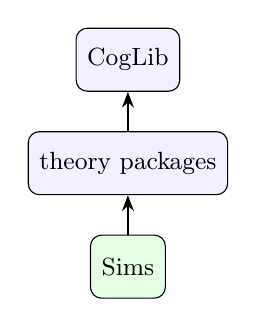
\begin{tikzpicture}[node distance=5mm, every node/.style={font=\small}]
      \node[box] (lib) {CogLib};
      \node[box, below=of lib] (th) {theory packages};
      \node[box, below=of th, fill=green!10] (sims) {Sims};
      \draw[arr] (th) -- (lib);
      \draw[arr] (sims) -- (th);
    \end{tikzpicture}
    \column{0.48\linewidth}
    \small
    \begin{itemize}
      \item A separate package; arrows point one way: nothing in the library or theories imports it.
      \item A \textbf{seeded} generator: every run reproducible.
      \item \textbf{Exact} draws: a uniform $k/10^9$ against the exact cumulative probabilities; no floating point in sampling.
      \item Programs: \code{lake exe sc-check}, \code{lake exe sc-learning}.
    \end{itemize}
  \end{columns}
\end{frame}
\note{
The simulations live in their own package, Sims, which depends on the library and the theories, while nothing depends on it, so the proofs, the theory matrix and the catalog never see simulation code. The generator is seeded, so every run is reproducible. And the draws are exact: a uniform rational is compared with the model's exact cumulative probabilities, with no floating point in sampling at all. There are two programs so far: one checks the sampler, one runs the learning simulation.
}

\begin{frame}{First, check the sampler against the model}
  \begin{itemize}
    \item A trial is drawn stage by stage, using the model's own retrieval, elaboration and learning; counting object by object.
    \item On small cases, compare every outcome's frequency with its \emph{exact} probability under the model's \code{trial}:
  \end{itemize}
  \begin{center}
  \begin{tabular}{lcc}
    \toprule
    Case (40{,}000 draws each) & worst $|z|$ & within $4\sigma$\\
    \midrule
    $1+1$, search length 1, criterion .3 & 1.30 & yes\\
    $1+2$, search length 2, criterion .2 & 1.60 & yes\\
    $2+2$, search length 3, criterion .5 & 1.25 & yes\\
    \bottomrule
  \end{tabular}
  \end{center}
  So the simulation draws from the model, not from an approximation of it.
\end{frame}
\note{
Before trusting a long run, check the sampler. A trial is drawn stage by stage, using the model's own retrieval, elaboration and strengthening; only counting is drawn object by object, because the model's full counting distribution is exponential in the sum. Then, on small cases where the exact distribution is easy to compute, every outcome's sampled frequency is compared with its exact probability under the model's trial. All are well within four standard errors, the worst at one point six. So the simulation draws from the model itself.
}

\begin{frame}{The simulation in the 1984 chapter (pp.~272--275)}
  \small
  \textbf{Specified}:
  \begin{itemize}
    \item answers 1--12, every association initially .01;
    \item 2000 learning trials; the 25 problems presented by parental input (Table 9.5), plus a constant;
    \item on each trial, a criterion from .05--.99 and a search length from 1--3, at random;
    \item elaboration adds .05; a counting-string prime on ascending and tie problems;
    \item learning: twice the increment for correct answers.
  \end{itemize}
  \textbf{Not given, so parameters here}: the prime's size, the increment, the counting error rates, the presentation constant ($c = 12$ reproduces the stated 5.4\% for $4+1$).
\end{frame}
\note{
Here's what the 1984 chapter specifies about its simulation: twelve possible answers, each starting with a weak association; two thousand learning trials, with problems presented in proportion to how often parents presented them; a random confidence criterion and search length on each trial; elaboration; a prime from the counting string; and twice the learning increment for correct answers. Some numbers aren't given: the size of the prime, the increment, the counting error rates, and the constant added to the presentation frequencies. Those become parameters, and a constant of twelve reproduces the frequencies the chapter does state.
}

\begin{frame}{Searching the unspecified parameters}
  \small
  Mean $|$difference$|$ from Fig.~9.8's peaks and shares (10 runs each):
  \begin{center}
  \begin{tabular}{lccccc}
    \toprule
    increment $\backslash$ prime & .01 & .02 & .05 & .1 & .2\\
    \midrule
    1/400 & .18 & .18 & .18 & .18 & .18\\
    1/250 & .11 & .10 & .10 & .09 & .08\\
    1/200 & .10 & .09 & .09 & .08 & \textbf{.06}\\
    1/150 & .18 & .17 & .18 & .17 & .14\\
    1/100 & .43 & .42 & .44 & .41 & .40\\
    \bottomrule
  \end{tabular}
  \end{center}
  An increment near 1/200 fits; faster learning overshoots. The fit improves with a \emph{larger} prime.
\end{frame}
\note{
Since some parameters aren't given, I searched them coarsely, comparing with the peaks and shares in the chapter's Figure 9.8. An increment around one two-hundredth fits best; faster learning overshoots badly, slower undershoots. And the fit keeps improving as the prime gets larger. This is a coarse sweep, not a fit, and I'll come back to what it suggests about the prime.
}

\begin{frame}{Against Fig. 9.8, after 2000 trials}
  \begin{center}
  \begin{tabular}{lcccc}
    \toprule
    Problems (effect) & Peak & Chapter & Share & Chapter\\
    \midrule
    $1+4$ vs $2+3$ (counting string) & .54 vs .40 & .67 vs .37 & .75 vs .61 & .77 vs .46\\
    $4+1$ vs $3+2$ (frequency) & .85 vs .55 & .80 vs .51 & .78 vs .71 & .76 vs .69\\
    $3+4$ vs $4+5$ (sum) & .31 vs .32 & .39 vs .32 & .55 vs .52 & .50 vs .43\\
    \bottomrule
  \end{tabular}
  \end{center}
  \small
  Increment 1/200, prime .2, counting errors .05; means over 20 runs. Peak: strength at the correct answer. Share: its fraction of the total.
\end{frame}
\note{
Here are the results at the best setting, against the chapter's three comparisons. Frequency of presentation: four plus one against three plus two, eighty-five against fifty-five, close to the chapter's eighty against fifty-one. The counting string: one plus four against two plus three, in the right direction, though the gap in peaks is smaller than the chapter's. And the sum of the addends: three plus four against four plus five, essentially tied, where the chapter shows a clear advantage for the smaller sum.
}

\begin{frame}{What reproduces, and what does not}
  \begin{itemize}
    \item \textbf{Frequency}: reproduced closely, at every setting tried.
    \item \textbf{Counting string}: reproduced in direction, but only with a large prime, .2, four times the elaboration's .05. The chapter does not give its size; this suggests it was large.
    \item \textbf{Sum}: not reproduced at any setting tried (primes to .4; counting errors .02--.1). Possible reasons:
    \begin{itemize}
      \item Table 9.5, as read from the scan, gives $4+5$ slightly more input than $3+4$; the text says equal. Some cells are faint.
      \item The chapter's values are from one simulated run; these are means over 20.
      \item Unspecified details: a continuous criterion, the prime during elaboration, the form of counting errors.
    \end{itemize}
  \end{itemize}
\end{frame}
\note{
So: the frequency effect comes out closely everywhere. The counting-string effect comes out in direction, but only if the prime is large, four times the size of elaboration; the chapter never gave the prime's size, so this is a small inference about the original. And the sum effect doesn't come out at any setting I tried. There are three candidate reasons. My reading of the parental-input table from the scan gives four plus five slightly more input than three plus four, where the text says they're equal, and some cells are faint. The chapter's numbers are from a single simulated run, while mine are averages. And there are details the chapter doesn't specify. Each of these is checkable.
}

\begin{frame}{What this adds, and next}
  \begin{itemize}
    \item \textbf{One implementation}, proved about and run; a sampler checked against the exact model before any long run.
    \item \textbf{Replications become specific}: where a published simulation leaves numbers out, the sweep shows which values matter, and what they must have been.
    \item \textbf{Disagreements become questions}: the sum effect points at a table, a single run, or an unstated detail.
  \end{itemize}
  \medskip
  Next: run-to-run spread; recheck Table 9.5; the test phase (Fig.~9.2A); then the multi-digit model learning as a whole.
\end{frame}
\note{
What does this add? One implementation that is both proved about and run, with the sampler checked against the exact model before any long run is trusted. Replications become specific: where a published simulation leaves numbers out, a sweep shows which ones matter and what they must have been, like the size of the prime. And disagreements become concrete questions, here about a table, a single run, or an unstated detail. Next: the spread across runs, a clean copy of the parental-input table, the chapter's test phase, and then the multi-digit model learning as a whole, recognition, associations and problem solving together.
}

\end{document}
